\documentclass[12pt]{article}
\usepackage{graphicx}
\usepackage{psfrag}
\usepackage{epsfig}
\usepackage{subfigure}
\usepackage{amssymb,amsmath}
\usepackage{verbatim}

%\usepackage{doublespace}

\textheight 23cm \topmargin -1cm \leftmargin 0cm

\marginparwidth 0mm    % Largeur des notes marge de droite
\textwidth 16.5cm      % Largeur du texte
\hsize \textwidth      % Longueur d'une ligne
\advance \hsize by -\marginparwidth
\oddsidemargin -4mm    % Marge gauche pages de droite - 1 inch (2.54 cm)
\evensidemargin \oddsidemargin % Idem pour les pages de gauche

\advance\hoffset by 5mm % Pour corriger un decalage residuel sur la gauche

\renewcommand{\hat}{\widehat}
\newcommand{\R}{\mathrm{I\!R\!}}
\newcommand{\C}{\mathrm{I\!\!\!C\!}}
\newcommand{\sinc}{\mbox{sinc}}
\newcommand{\diag}{\mbox{diag}}
\newcommand{\Tr}{\mbox{Tr}}

% commands
\newtheorem{theo}{Theorem}
\newtheorem{proposition}{Proposition}
\newcommand{\nc}{\newcommand}
\nc{\RR}{\mbox{\rm I$\!$R}} \nc{\dsp}{\displaystyle}
\nc{\Div}{\mbox{\rm div }} \nc{\beequ}{\begin{equation}}
\nc{\barr}{\begin{array}} \nc{\earr}{\end{array}}
\nc{\eequ}{\end{equation}} \nc{\BFF}{\hbox{\boldmath{${\cal
F}$}}^{(j)}({\bf y}^s,t)}

\nc{\hr}{\widehat{r}} \nc{\hh}{\widehat{h}} \nc{\hs}{\widehat{s}}
\nc{\hn}{\widehat{n}} \nc{\hw}{\widehat{w}} \nc{\hd}{\widehat{d}}
\nc{\hG}{\widehat{\Gamma}} \nc{\om}{\omega} \nc{\yy}{{\bf y}}
\nc{\ys}{{\bf y}^s} \nc{\yo}{{\bf y}_0} \nc{\xp}{{\bf x}_p}
\nc{\xr}{{\bf x}_r} \nc{\co}{{\cal O}}
\renewcommand\labelenumi{\alph{enumi})}
\begin{document}
\begin{center}
\textbf{Practice Set 1 Solutions}
\end{center}
\paragraph{Problem 1}

\begin{enumerate}
\item Assume $G_t=G_r=1$ 
\begin{eqnarray*}
P_t(watts)&=&10^{(42-30)/10}=15.8489\\
P_r&=&P_t\left(\frac{h_th_r}{d^2}\right)=1.4264e^{-10}\\
P_r(dBm)&=&10log_{10}(P_r)+30=-68.4576dBm
\end{eqnarray*}
\item Set $P_r(dBm)=-90dBm$ and find $d$ which is $6.9km$
\item
\verbatiminput{pl.m}
See Figure~\ref{fig:pl} for output.
\begin{figure}
    \centering
  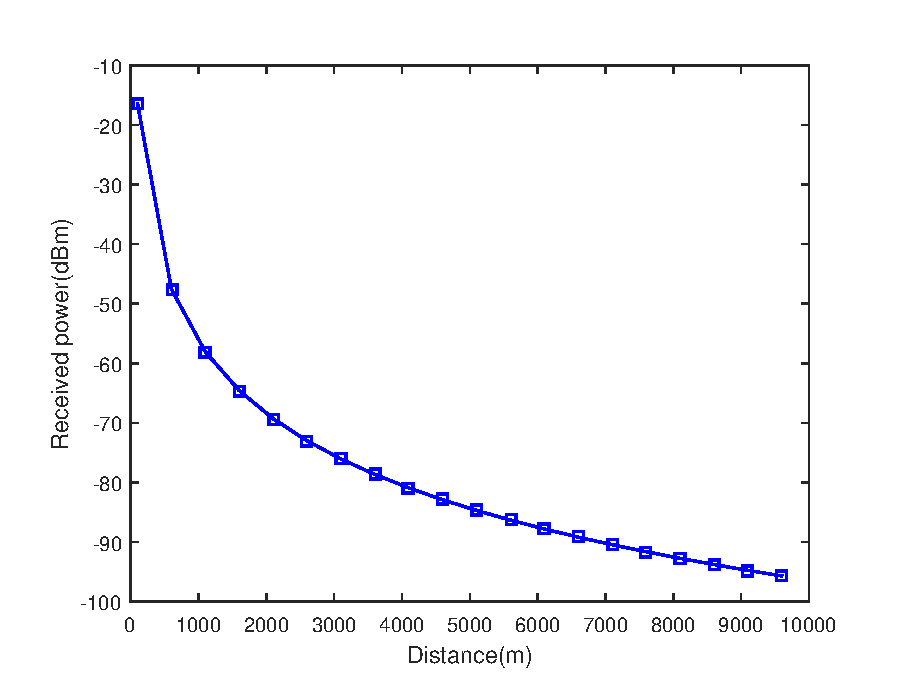
\includegraphics[width=4.0in]{pl.eps}\\
  \caption{Distance Vs Received power (dBm)}\label{fig:pl}
\end{figure}
\end{enumerate}


\paragraph{Problem 2}
\begin{enumerate}
\item
\begin{eqnarray*}
E\left[U(\tau,\nu_1)U^*(\tau,\nu_2)\right]&=&
E\left[\int_{-T_u/2}^{T_u/2}\int_{-T_u/2}^{T_u/2}p(\tau,t)p^*(\tau,t')e^{-j2\pi(\nu_1t-\nu_2t')}dtdt'\right]\\
&=&\int_{-T_u/2}^{T_u/2}\int_{-T_u/2}^{T_u/2}E\left[p(\tau,t)p^*(\tau,t')\right]e^{-j2\pi(\nu_1t-\nu_2t')}dt
dt'
\end{eqnarray*}
by the stationarity assumption we have:
\begin{eqnarray*}
E\left[U(\tau,\nu_1)U^*(\tau,\nu_2)\right]=
\int_{-T_u/2}^{T_u/2}\int_{-T_u/2}^{T_u/2}R_t(\tau,t'-t)e^{-j2\pi(\nu_1t-\nu_2t')}dt
dt'
\end{eqnarray*}
Let $\Delta t=t'-t$ and $T_u\rightarrow\infty$:
\begin{eqnarray*}
E\left[U(\tau,\nu_1)U^*(\tau,\nu_2)\right]&=&
\int_{\mathbb{R}}\int_{\mathbb{R}}R_t(\tau,\Delta
t)e^{-j2\pi(\nu_1t-\nu_2\Delta t-\nu_2t)}dt d\Delta t\\
&=&\mathcal{F}^{-1}_{\Delta t}\left\{R_t(\tau,\Delta
t)\right\}(\nu_2)\int_{\mathbb{R}}e^{-j2\pi(\nu_1-\nu_2)t}dt
\end{eqnarray*}
where $\mathcal{F}_k^{-1}\{f(k)\}(x)=\int_{-\infty}^\infty f(k) e^{2\pi i kx}dk$ is the Inverse Fourier Transform
operator with respect to the appropriate variable.  The last
integral is just the Fourier Transform of a complex exponential
evaluated at zero frequency: $\delta(f+\nu_1-\nu_2)|_{f=0}$.
Thus,
\begin{eqnarray*}
E\left[U(\tau,\nu_1)U^*(\tau,\nu_2)\right]&=&
\mathcal{F}^{-1}_{\Delta t}\left\{R_t(\tau,\Delta
t)\right\}(\nu_2)\delta(\nu_1-\nu_2)
\end{eqnarray*}
And we are done!
\item
\begin{eqnarray*}
E\left[P(f,t)P^*(f+\Delta
f,t)\right]&=&\int_{\mathbb{R}}\int_{\mathbb{R}}E\left[p(\tau_1,t)p^*(\tau_2,t)\right]e^{j2\pi\left[f\tau_1-(f+\Delta
f)\tau_2\right]}d\tau_1d\tau_2\\
&=&\int_{\mathbb{R}}E\left[|p(\tau_2,t)|^2\right]e^{-j2\pi\Delta
f\tau_2}d\tau_2\\
&=&R_f(\Delta f,t)
\end{eqnarray*}
The last equality follows since the integral above it is only a
function of $\Delta f$.
\end{enumerate}

\paragraph{Problem 3}
\verbatiminput{ray.m}
See Figure~\ref{fig:ray} for output.
\begin{figure}
  % Requires \usepackage{graphicx}
  \centering
  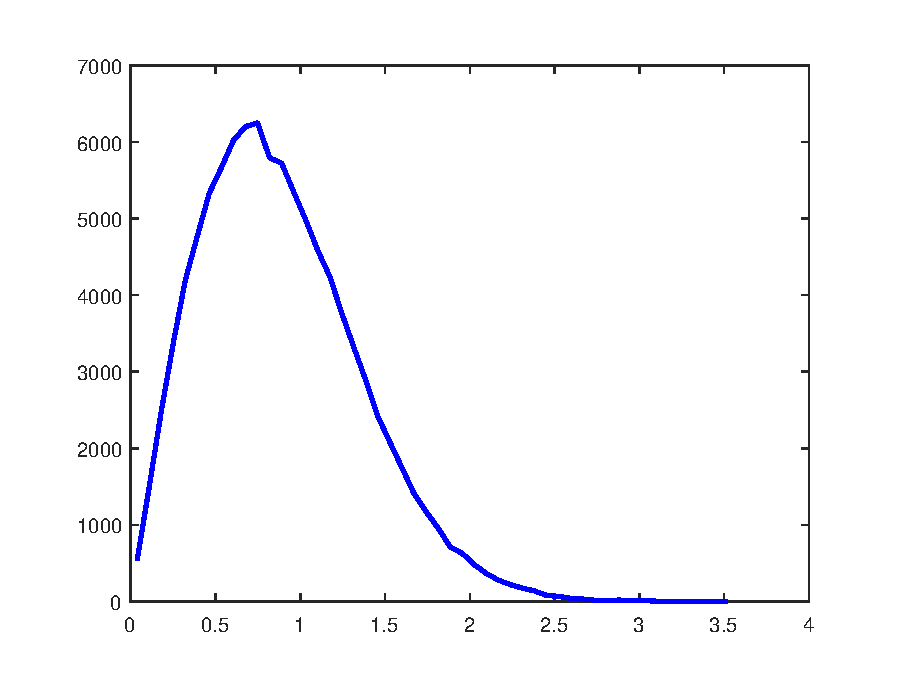
\includegraphics[width=4.0in]{ray.eps}\\
  \caption{Raleigh pdf}\label{fig:ray}
\end{figure}

\paragraph{Problem 4}
\verbatiminput{ric.m}
See Figure~\ref{fig:ric} for output.
\begin{figure}
    \centering
  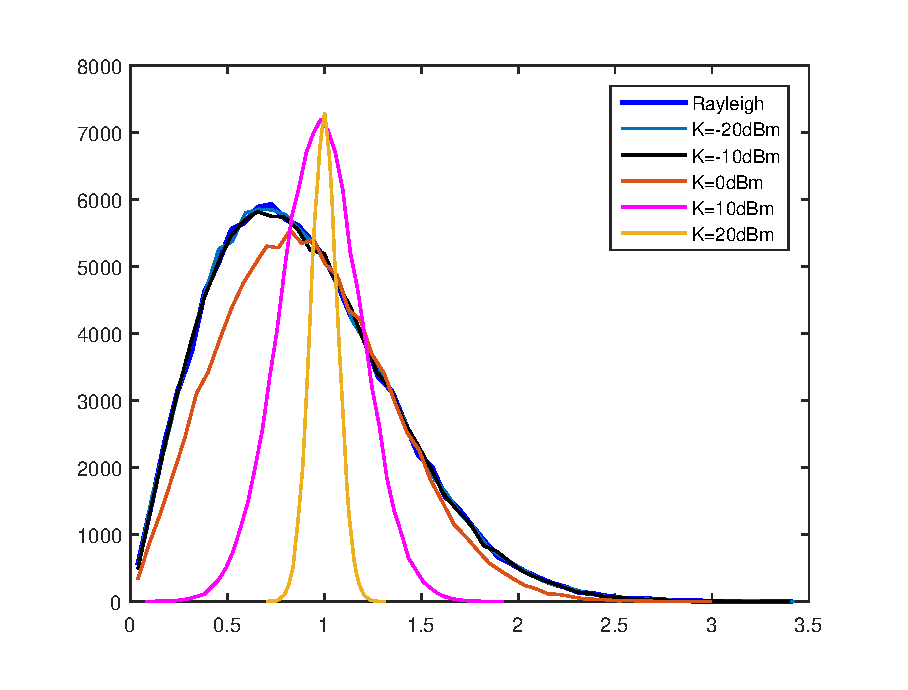
\includegraphics[width=4.0in]{ric.eps}\\
  \caption{Rician and rayleigh pdfs}\label{fig:ric}
\end{figure}
\paragraph{Problem 5}
\verbatiminput{Hiid.m}
\paragraph{Problem 6}
\verbatiminput{H_corr.m}
\paragraph{Problem 7}
\verbatiminput{mimoRic.m}
\paragraph{Problem 8}
\begin{enumerate}
\item
\begin{eqnarray*}
{\bf H}[k]&=&{\bf H}_1g(kT_s)+{\bf H}_2g(kT_s-\tau_1)\\
&=&\frac{\mbox{sinc}\left(k\right)\cos\left(\pi\beta
k\right)}{1-4\beta^2 k^2}{\bf H}_1+
\frac{\mbox{sinc}\left(k-\tau_1/T_s\right)\cos\left(\pi\beta
(k-\tau_1/T_s)\right)}{1-4\beta^2 (k-\tau_1/T_s)^2} {\bf H}_2
\end{eqnarray*}

\item  The following script produces the desired results:
\verbatiminput{q3.m}
%\verbatiminput{q3_output.m}
\end{enumerate}
\end{document}

















